%
% File: chap01.tex
% Author: ta16969
% Description: The objective here is an introductory pre-amble, which sets the tone and concludes with a tentative structure of the how the report will be developed along the way
%
%
\let\textcircled=\pgftextcircled
\chapter{Introduction}
\label{chap:intro}

\initial{T}eaching practices in recent years, particularly those relevant to Computer Science (CS), at a primary and secondary schooling level seems to have had a coming of age in the UK \cite{bbcCS1970}. This may be driven by a growing market and stakeholder appetite, as relevant technologies mature and therefore require a reliable stream of skilled technical workers \cite{edugovUK,guardianCSEducation}.

However despite growing demand, relevance and resources dedicated towards CS education at a primary and secondary schooling level, existing teaching resources are stretched because of a myriad of reasons, beyond the scope of this report\cite{guardianTeachingShortage,telegraphTeachingShortage}. However it stands to reason that this likely results in the deterioration/failure of underlying pedagogical and social objectives.
Therein lies  an argument for 'flexible' and innovative pedagogies \cite{heaTelDefinition}, which extends to Technology Enhanced Learning and Game Enhanced Learning.






%=======^Spaces dont really matter
\section{Technology Enhanced Learning (TEL)}
\label{sec:sec01}

 TEL is not a new concept and has been around for a while, masked by the fact that is constant evolving with advances in both technology and pedagogical trends \cite{UniTexAus}.In fact it has become synonymous  to refer to e-learning\cite{heaTelDefinition}.
 
 However beyond it's inherent legacy,it is a key theme in emergent 'flexible' pedagogies to create innovative new  practices \cite{heaTelDefinition}.Furthermore flexible pedagogical practices that incorporate TEL, have been demonstrably effective as substitutes and compliments to traditional practices in creating resource and cost savings \cite{govUKTELCostSavings}
 
 Therefore it can be reasoned that TEL may provide a solution for teaching CS, in an age where relevant skills are in high demand but resources may not be readily available, within the context of traditional pedagogical approaches.
 
\subsection{Game Enhanced Learning (GEL)}
Enhanced pedagogical practices that are delivered via digital games are considered by some as an emerging research area in the field of TEL, i.e.otherwise referred to as Game Enhanced Learning (GEL) \cite{GEL}, which is the underlying theme of this report.
\label{subsec:subsec01}
\begin{figure}[h]
    \centering
    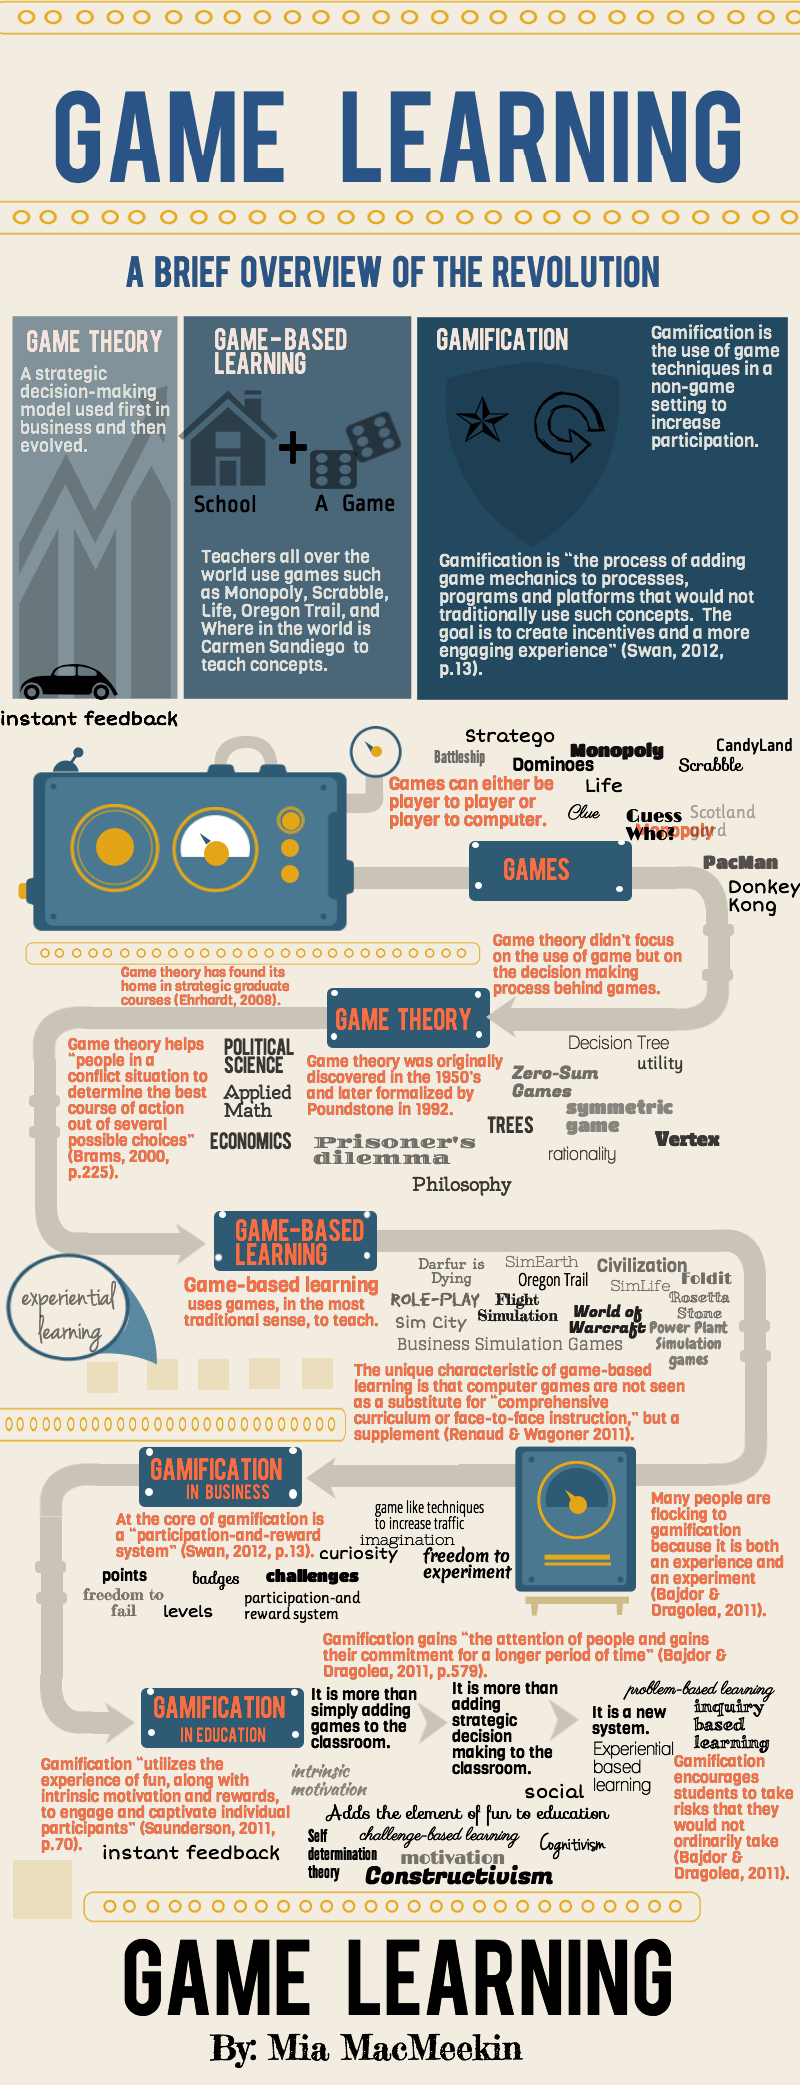
\includegraphics[scale=0.22]{fig01/GELInfograph}
    \caption{Infographic: Game Enhanced Learning}
    \label{fig:my_label}    
\end{figure}
The next few chapter's encompass the development and finished product of Team Emu's software engineering project; i.e. the development of a video game to teach children programming skills utilising GEL.

%=========================================================